%!TEX root = thesis.tex

\chapter{Introduction}
\label{chap:introduction}

\begin{chapquote}{Frederick Brooks, \textit{The Mythical Man-Month}, p.185}
``In spite of progress in restricting and simplifying the structures of software, they remain inherently unvisualizable, thus depriving the mind of some of its most powerful conceptual tools. This lack not only impedes the process of design within one mind, it severely hinders communication among minds.''
\end{chapquote}

Visualisations bridge the gap between understanding and enjoyment. \more

In software, visualisations have attempted to provide a higher level of understanding but have rarely been effective in communicating the fundamental processes of software development. The Mythical Man-Month goes so far as to suggest that ``software is invisible and unvisualizable''\cite{Brooks1995} sparking debate as to the effectiveness of all software visualisations used in the understanding of software.

Within the last two decades, the introduction and development of ``live coding'' has presented a unique application space for visualisations and the potential for effective communication directly with audiences. These new developments could challenge the long-held belief that ``software is invisible and unvisualizable''.

The intention of software visualisations is to communicate software effectively. In recent years there has been a push to develop effective software visualisations as the audience of software becomes more diverse, multidisciplinary teams within the industry become the standard, and multimedia and the arts become more focussed on effective software development. Live coding presents a space in which a wide audience and dynamic software is common and presents a space in which visualisations could provide significant benefit to the experience of observers. Live coding is a means of combining the artistic goal of enjoyment and the educational aspects associated with programming with visualisations to effectively communicate software.

This thesis investigates the proposition that ``code visualisation improves the experience of observers'' in the setting of a live arts practice. More specifically, this thesis investigates the question: ``can the application of visualisation techniques to live coding enhance audience experience by increasing understanding and enjoyment?''. These questions were examined through a process of prototype development, user study evaluation and refinement.

The application of software visualisations to the process of live coding has been explored. A process of design iteration and evaluation was conducted in collaboration with a live coding  artist to develop software visualisations. Three studies were administered, including one field study and two laboratory studies as a means to determine if understanding and enjoyment could be influenced by the introduction of visualisations to live coding.

\section{Background}

For most of its history, source code has been displayed as simple text. This is due to the expressiveness of the text format and despite its inefficiencies. It is only recently, due to ever increasing programming language complexity, increasing screen fidelity and increasing computational power, that code annotations and syntax highlighting have become more commonplace. Nevertheless, these visual enhancements rarely provide information beyond the basic grammar of the language they are intended to augment. The limitations of this approach are becoming ever more apparent as programming languages and interactive programming environments move towards the need for real-time comprehension and a need to understand the source code within the context of a running program.

A number of modern software environments are supporting the concept of hotswapping source code. Within software environments, hotswapping refers to the process of modifying program source code at runtime to achieve desired behaviour without interrupting or restarting the system. Examples of languages and platforms supporting this workflow include Java with HotSwap or JRebel~\cite{ZeroTurnaround2014} and Python, in addition to a variety of other custom platforms and modifications (e.g.~\cite{Thomas2011}). This workflow has also inspired the programming practice of ``live coding''. 

Live coding further develops the concept of hotswapping source code, applying it to live musical and visual performance. In live coding a programmer performs for an audience. The audience observes the programmer as they modify an active program to produce music and visuals. Some of the most important and influential live coding environments over the last decade have included SuperCollider~\cite{McCartney}, ChucK~\cite{Wang2008} and Extempore~\cite{Sorensen}. These environments have a growing following as the field of live coding matures.

\section{Related Work}

A number of existing software visualisation techniques exist. Some of the most common software visualisations include static diagrams~\citetemp{x} and syntax highlighting (see Figure~\ref{fig:syntax-highlighting}). These techniques generally model the structure of the program to allow for more effective navigation around structures and take advantage of visual memory.

While diagrams and syntax highlighting provide information regarding the structure of source code, the fundamental nature of software is to change~\citetemp{mythical man-month?}. Understanding these changes requires visualising the software development process. Techniques to visualise the changes occurring during software development process include Gource~\cite{Caudwell2010} (Figure~\ref{fig:gource}) and Code Swarm~\cite{Ogawa2012} (Figure~\ref{fig:code-swarm}). These visualisation techniques show historic source code changes, based on source code respository data.


\begin{figure}
\centering
\begin{subfigure}{.5\textwidth}
  \centering
  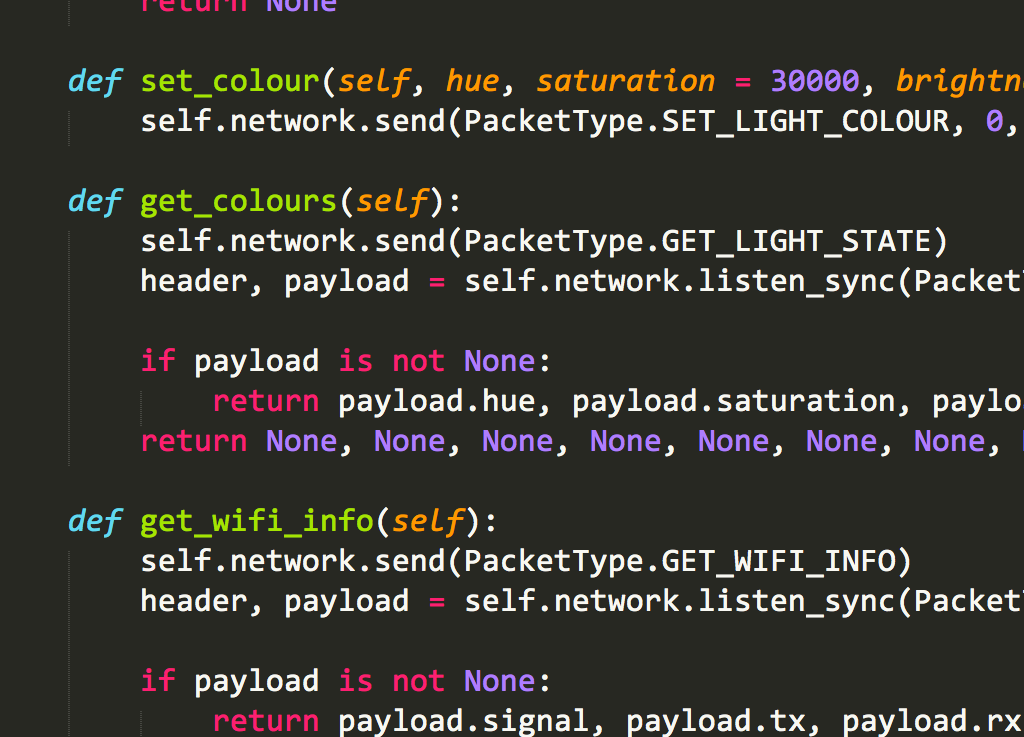
\includegraphics[width=.95\linewidth]{../images/code-visualisations/syntax-highlighting.png}
  \caption{Syntax Highlighting}
  \label{fig:syntax-highlighting}
\end{subfigure}%
\begin{subfigure}{.5\textwidth}
  \centering
  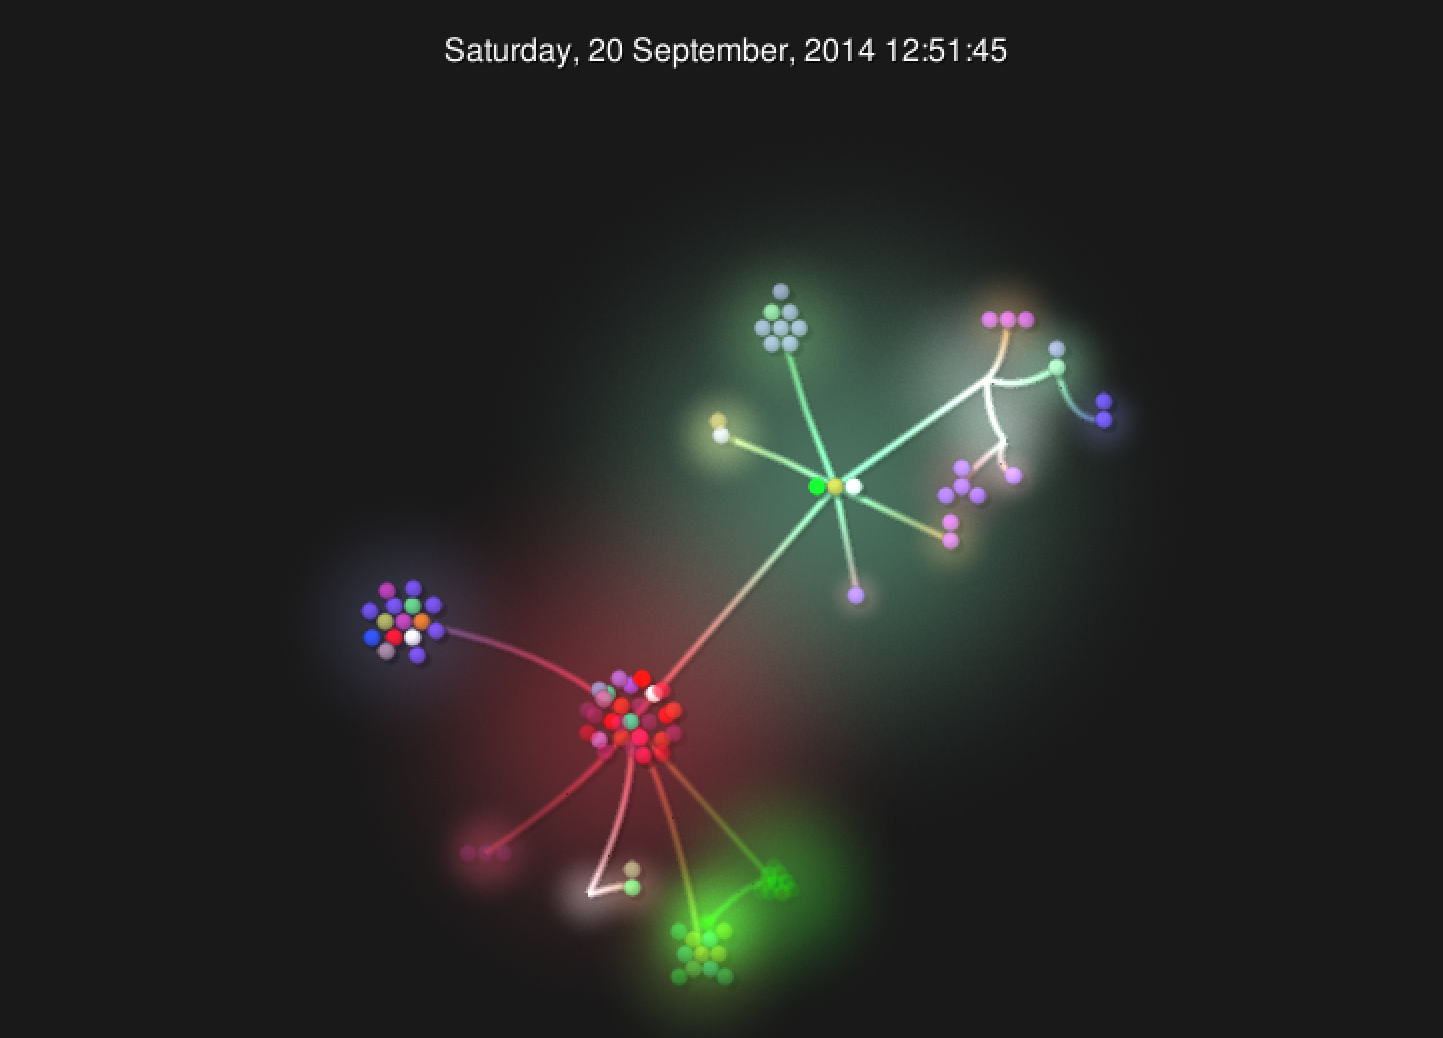
\includegraphics[width=.95\linewidth]{../images/code-visualisations/gource.png}
  \caption{Gource}
  \label{fig:gource}
\end{subfigure}\\
\begin{subfigure}{.5\textwidth}
  \centering
  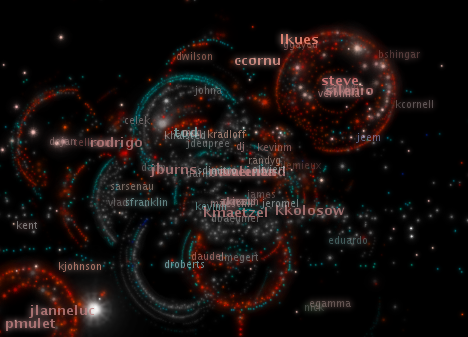
\includegraphics[width=.95\linewidth]{../images/code-visualisations/code-swarm.png}
  \caption{Code Swarm}
  \label{fig:code-swarm}
\end{subfigure}%
\begin{subfigure}{.5\textwidth}
  \centering
  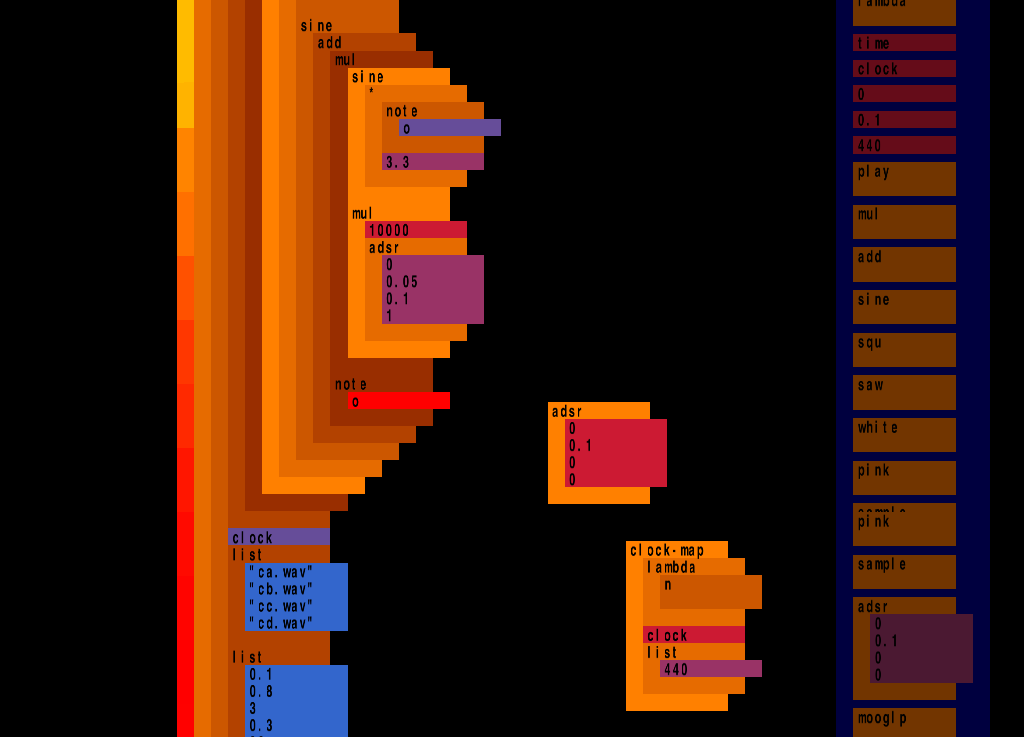
\includegraphics[width=.95\linewidth]{../images/code-visualisations/scheme-bricks.png}
  \caption{Scheme Bricks}
  \label{fig:scheme-bricks}
\end{subfigure}

\caption{Existing software visualisations.}
\label{fig:code-visualisations}
\end{figure}

Showing historic source code changes allows the process of programming to be understood. However, this information is not immediately useful to programmers or observers. Visualisation of active software has shown potential in providing useful and interesting information, allowing the programmer to take actions based on the visualisations and allowing the observers to make relevant judgement of what actions the programmer is taking. Visualisation techniques such as inline annotations~\cite{Swift2013} provide direct feedback directly useful to both the programmer and observers, and technologies such Light Table~\cite{Kodowa2014} with an inline interactive terminal or \ac{REPL} have further identified how useful visual feedback can be.

Techniques of visualising active software is directly relevant to live coding. Examples of existing software visualisations within live coding include Scheme Bricks (Figure~\ref{fig:scheme-bricks}) and a number of others (see~\cite{McLean2010a} for a review). These visualisation techniques suggest potential within live coding for effective process-driven visuals intending to enhance the observer's experience. However, no systematic studies of process-driven visualisations have been conducted within live coding.



\section{Structure}

The structure of this thesis consists of Chapter~\ref{chap:literature-review} summarising the literature including the basis for and the direction of this thesis. Following this, Chapter~\ref{chap:exploratory-field-study} discusses the initial exploratory field study conducted to investigate existing perception and understanding of the live coding process. Chapter~\ref{chap:visualisation-design} discusses the first iteration of the visualisation prototype developed following the results of the exploratory field study. Chapter~\ref{chap:user-study} summarises the first user study conducted with the visualisation prototype. Chapter~\ref{chap:visualisation-refinement} discusses refinement of the visualisation prototype motivated by the results of the first user study. Chapter~\ref{chap:follow-up-user-study} discusses the follow-up user study conducted to analyse the refined visualisations. Chapter~\ref{chap:summary} summarises the results of the user studies, contributions, limitations and future work. Finally, Chapter~\ref{chap:conclusion} provides some final words to conclude the thesis.

